\documentclass[12pt,a4paper]{report}

% ---------- Packages ----------
\usepackage[a4paper,left=1.3in,right=0.9in,top=0.85in,bottom=0.85in]{geometry}
\usepackage[T1]{fontenc}
\usepackage{mathptmx}             % Times New Roman-equivalent text + math font
\usepackage{graphicx}
\usepackage{booktabs}
\usepackage{array}
\usepackage{caption}
\usepackage{float}
\usepackage{xcolor}
\usepackage{titlesec}
\usepackage{fancyhdr}
\usepackage{enumitem}
\usepackage{hyperref}
\usepackage{tikz}
\usetikzlibrary{shapes,arrows.meta,positioning}
\usepackage{tabularx}
\usepackage{setspace}
\usepackage{amssymb}

\definecolor{navy}{RGB}{21,42,79}
\definecolor{accent}{RGB}{37,99,235}

\titleformat{\chapter}[hang]{\normalfont\Large\bfseries\color{navy}}{\thechapter.}{12pt}{\Large}
\titlespacing*{\chapter}{0pt}{-14pt}{14pt}
\titleformat{\section}{\normalfont\large\bfseries\color{navy}}{\thesection}{8pt}{}
\titleformat{\subsection}{\normalfont\normalsize\bfseries}{\thesubsection}{6pt}{}

\setlength{\headheight}{14pt}
\pagestyle{fancy}
\fancyhf{}
\fancyhead[L]{\small\nouppercase{\leftmark}}
\fancyhead[R]{\small\thepage}
\renewcommand{\headrulewidth}{0.4pt}
\fancypagestyle{plain}{\fancyhf{}\fancyhead[L]{\small\nouppercase{\leftmark}}\fancyhead[R]{\small\thepage}\renewcommand{\headrulewidth}{0.4pt}}

\hypersetup{
    colorlinks=true,
    linkcolor=navy,
    citecolor=navy,
    urlcolor=accent,
    pdftitle={Used Car Price Prediction and Analysis System Using Machine Learning},
    pdfauthor={Bankar Smitraj Dinkar}
}

\setlength{\parindent}{0pt}
\setlength{\parskip}{5pt}
\setstretch{1.05}

\newcommand{\imgpath}{.}

% Tables/figures stay single-spaced even though body text is 1.5-spaced --
% standard practice, keeps tabular data compact and legible.
\let\oldtable\table
\let\endoldtable\endtable
\renewenvironment{table}[1][H]{\oldtable[#1]\singlespacing}{\endoldtable}

\begin{document}
\pagenumbering{roman}

% =========================================================
% TITLE PAGE
% =========================================================
\begin{titlepage}
\centering
\thispagestyle{empty}
\vspace*{0.1cm}

\includegraphics[width=2.1cm]{images/college_logo.png}\\[4pt]
{\large\bfseries Sanjivani College of Engineering, Kopargaon\par}
{\normalsize Department of Computer Engineering\par}
{\normalsize (Affiliated to Savitribai Phule Pune University, Pune)\par}
\vspace{0.25cm}
\rule{\linewidth}{0.8pt}

\vspace{0.55cm}
{\Huge\bfseries\color{navy} Used Car Price Prediction\\[4pt] and Analysis System\\[4pt] Using Machine Learning\par}
\vspace{0.3cm}
{\large A Mini Project Synopsis Submitted in Partial Fulfilment\\
of the Requirements for the Course\par}
\vspace{0.2cm}
{\Large\bfseries HOCO492 --- Mini Project: Artificial Intelligence and Machine Learning\par}

\vspace{0.65cm}
{\large\itshape Submitted by\par}
\vspace{0.2cm}
{\LARGE\bfseries Bankar Smitraj Dinkar\par}
{\large Roll No.: 09 \quad\textbar\quad PRN No.: UCS23M1009\par}

\vspace{0.65cm}
{\large\itshape Under the Guidance of\par}
\vspace{0.2cm}
{\Large\bfseries Prof. Bhagyashri Bhagawan Kotame\par}
{\large Assistant Professor, Department of Computer Engineering\par}

\vfill
{\large Department of Computer Engineering\par}
{\large Sanjivani College of Engineering, Kopargaon\par}
{\large Academic Year 2026--2027\par}
\end{titlepage}

% =========================================================
% CERTIFICATE
% =========================================================
\chapter*{Certificate}
\thispagestyle{empty}

This is to certify that the mini project report entitled \textbf{``Used Car
Price Prediction and Analysis System Using Machine Learning''} is a bona
fide work carried out by \textbf{Bankar Smitraj Dinkar} (Roll No.
\textbf{09}, PRN No. \textbf{UCS23M1009}) in partial fulfilment of the
requirements for the course \textbf{HOCO492 --- Mini Project: Artificial
Intelligence and Machine Learning}, during the academic year
\textbf{2026--2027}.

The work presented in this report is the result of the candidate's own
investigation and has not been submitted elsewhere for the award of any
other degree or diploma.

\vspace{1.6cm}
\begin{minipage}[t]{0.45\linewidth}
\textbf{Prof. Bhagyashri Bhagawan Kotame}\\
Project Guide, Assistant Professor\\
Department of Computer Engineering
\end{minipage}
\hfill
\begin{minipage}[t]{0.45\linewidth}
\textbf{[Head of Department Name]}\\
Head of Department\\
Department of Computer Engineering
\end{minipage}

\vspace{1.6cm}
\noindent Date: \underline{\hspace{4cm}} \hfill Place: Kopargaon

\vspace{1cm}
\section*{Acknowledgement}
I would like to express my sincere gratitude to \textbf{Prof. Bhagyashri
Bhagawan Kotame}, Assistant Professor, Department of Computer Engineering,
for her valuable guidance and continuous support throughout the
development of this mini project. I also thank the Department of Computer
Engineering, \textbf{Sanjivani College of Engineering, Kopargaon}, for
providing the resources and environment necessary to complete this work.

% =========================================================
% ABSTRACT
% =========================================================
\chapter*{Abstract}
\thispagestyle{empty}
Estimating a fair price for a used car is difficult without domain
expertise, as buyers and sellers typically rely on inconsistent manual
estimates or opaque dealer quotes. This project presents a complete,
reproducible machine-learning pipeline that predicts a used car's selling
price from its attributes (age, kilometers driven, fuel type,
transmission, engine capacity, mileage, power, seats, and ownership
history) using classical supervised regression. Six algorithms --- Linear
Regression, Ridge Regression, Decision Tree, Random Forest, Gradient
Boosting, and XGBoost --- were trained and objectively compared on a real,
public dataset of 8,128 CarDekho used-car listings using 5-fold
cross-validation, followed by bounded hyperparameter tuning of the two
strongest tree-based candidates with \texttt{RandomizedSearchCV}. The
final model, selected purely on held-out test-set performance, was
\textbf{Gradient Boosting}, achieving a test R\textsuperscript{2} of
\textbf{0.928} and a Mean Absolute Percentage Error of \textbf{21.3\%}.
The trained pipeline is deployed through an interactive Streamlit
application offering price prediction, dataset analytics, and model
performance dashboards, and is validated by 40 automated test cases
covering data integrity, preprocessing correctness, and prediction
reliability. The report documents every preprocessing decision, avoids
data leakage by design, and honestly discusses the system's limitations
rather than overstating its accuracy.

\textbf{Keywords:} Machine Learning, Regression, Used Car Price
Prediction, Random Forest, Gradient Boosting, Feature Engineering,
Streamlit, Scikit-learn.

% =========================================================
% TABLE OF CONTENTS / LIST OF FIGURES / LIST OF TABLES
% =========================================================
{\small\tableofcontents}

% List of Figures / List of Tables share the Contents page (plenty of
% blank space below a 9-entry TOC) instead of each forcing its own
% near-empty page via the default \listoffigures/\listoftables commands.
% \small keeps all three index lists on one page.
\begingroup\small
\makeatletter
\addcontentsline{toc}{chapter}{List of Figures}
\section*{\listfigurename}
\@starttoc{lof}

\addcontentsline{toc}{chapter}{List of Tables}
\section*{\listtablename}
\@starttoc{lot}
\makeatother
\endgroup

\clearpage
\pagenumbering{arabic}
\setcounter{page}{1}

% =========================================================
\chapter{Introduction}

Used-car pricing today is largely determined by informal estimation ---
dealer judgment, word-of-mouth comparison, or generic online calculators
that do not disclose their underlying methodology or accuracy. This lack
of transparency makes it hard for both buyers and sellers to trust a
quoted price.

This project applies \textbf{supervised machine learning regression} to
the problem: given a labeled dataset of real past used-car sales, a model
is trained to learn the relationship between a vehicle's observable
attributes and its actual selling price, and that learned relationship is
then used to estimate a fair price for a new listing.

\section*{Objectives}
\begin{itemize}[nosep]
    \item Acquire and validate a real, public used-car dataset.
    \item Build a leakage-free preprocessing and feature-engineering pipeline.
    \item Train and objectively compare multiple classical regression algorithms.
    \item Tune the strongest candidates and select a final model using held-out test performance.
    \item Deploy the trained pipeline behind an interactive, input-validated web application.
    \item Verify correctness and reliability with an automated test suite.
\end{itemize}

% =========================================================
\chapter{Literature Survey}

Five published studies on used-car and vehicle price prediction using
machine learning were reviewed to position this project's methodology
against prior work (Table~\ref{tab:litsurvey}).

\begin{table}[H]
\centering
\small
\begin{tabularx}{\textwidth}{@{}lX@{}}
\toprule
\textbf{Study} & \textbf{Method \& Key Finding} \\
\midrule
Pudaruth (2014) &
Linear regression, k-NN, na\"ive Bayes, decision trees on $\sim$200
Mauritian newspaper listings; 60--70\% accuracy, limited by small dataset
size. \\[4pt]
Monburinon et al. (2018), ICBIR &
Compared regression models on German used-car listings; gradient boosted
regression trees gave the best performance. \\[4pt]
Gegic et al. (2019), \textit{TEM Journal} &
ANN + SVM + Random Forest ensemble on Bosnian listings; ensemble
outperformed any single algorithm. \\[4pt]
Pal et al. (2018), FICC (Springer) &
Random Forest (500 trees); 95.82\% training vs. 83.63\% testing accuracy
--- a visible overfitting gap. \\[4pt]
Noor \& Jan (2017), \textit{IJCA} &
Multiple linear regression reported $\sim$98\% precision on a vehicle
listing dataset. \\
\bottomrule
\end{tabularx}
\caption{Summary of reviewed literature on used-car price prediction.}
\label{tab:litsurvey}
\end{table}

\textbf{Synthesis:} tree-based ensembles consistently outperform plain
linear regression for this problem across independent studies -- a
finding this project's own results (Chapter 5) reproduce independently on
a different dataset. Full citation details and per-paper relevance are
documented in \texttt{docs/literature\_survey.md}.

% =========================================================
\chapter{System Analysis and Design}

\section*{Existing vs. Proposed System}
\textbf{Existing systems} rely on manual/dealer estimation with no
reproducible methodology, or commercial valuation tools that do not
disclose their model, features, or error rate. \textbf{The proposed
system} is a transparent, documented ML pipeline that reports its own
accuracy, explains its price range methodology, and discloses its
limitations openly.

\section*{System Architecture}
\begin{figure}[H]
\centering
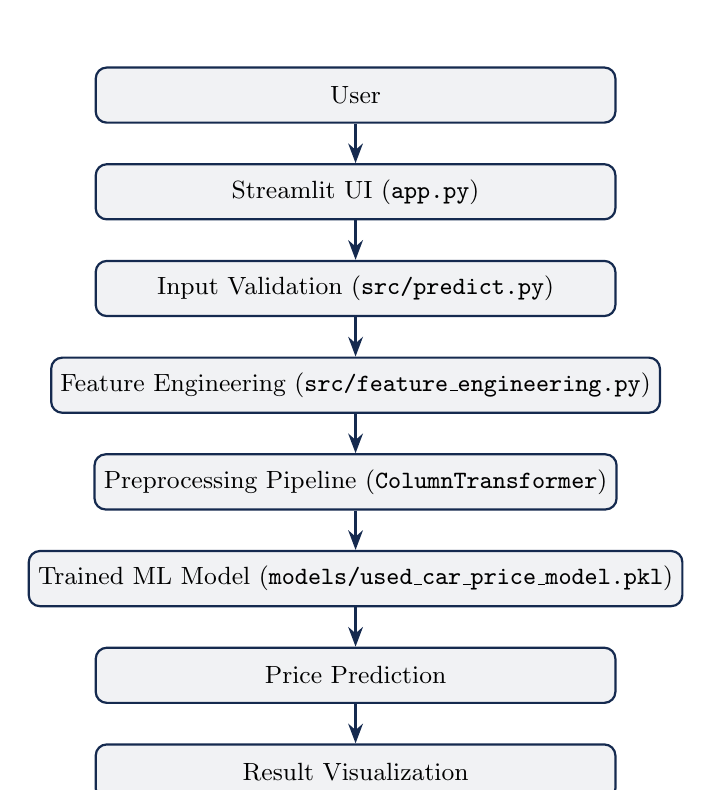
\begin{tikzpicture}[
    node distance=5mm,
    box/.style={rectangle, draw=navy, thick, rounded corners, fill=navy!6,
        minimum width=6.6cm, minimum height=0.7cm, align=center, font=\small},
    arr/.style={-{Stealth[length=2.5mm]}, thick, navy}
]
\node[box] (user) {User};
\node[box, below=of user] (ui) {Streamlit UI (\texttt{app.py})};
\node[box, below=of ui] (val) {Input Validation (\texttt{src/predict.py})};
\node[box, below=of val] (fe) {Feature Engineering (\texttt{src/feature\_engineering.py})};
\node[box, below=of fe] (pp) {Preprocessing Pipeline (\texttt{ColumnTransformer})};
\node[box, below=of pp] (model) {Trained ML Model (\texttt{models/used\_car\_price\_model.pkl})};
\node[box, below=of model] (pred) {Price Prediction};
\node[box, below=of pred] (viz) {Result Visualization};

\draw[arr] (user) -- (ui);
\draw[arr] (ui) -- (val);
\draw[arr] (val) -- (fe);
\draw[arr] (fe) -- (pp);
\draw[arr] (pp) -- (model);
\draw[arr] (model) -- (pred);
\draw[arr] (pred) -- (viz);
\end{tikzpicture}
\caption{System architecture: from user input to final result.}
\end{figure}

The system is organized into four layers: an \textbf{input layer}
(Streamlit form widgets), a \textbf{processing layer} (validation and
feature engineering), an \textbf{ML layer} (a single bundled
\texttt{scikit-learn Pipeline} combining preprocessing and the model), and
a \textbf{presentation layer} (prediction results and analytics
dashboards). Bundling preprocessing and the model together guarantees the
exact transformation learned at training time is applied at inference
time, eliminating train/serve skew.

% =========================================================
\chapter{Dataset and Methodology}

\section*{Dataset}
CarDekho used-car listings, \textit{``Car details v3.csv''}
(Kaggle: \texttt{nehalbirla/vehicle-dataset-from-cardekho}), consisting of
\textbf{8,128 raw rows} and \textbf{13 columns}: \texttt{name, year,
selling\_price, km\_driven, fuel, seller\_type, transmission, owner,
mileage, engine, max\_power, torque, seats}.

\section*{Data Cleaning}
\begin{itemize}[nosep]
    \item Duplicate rows removed (1,202 exact duplicates found).
    \item Units stripped from text-numeric columns, e.g.
    \texttt{"1248 CC"} $\rightarrow$ \texttt{1248.0},
    \texttt{"74 bhp"} $\rightarrow$ \texttt{74.0},
    \texttt{"23.4 kmpl"} $\rightarrow$ \texttt{23.4}.
    \item Rows with missing/non-positive \texttt{selling\_price} dropped (target cannot be imputed).
    \item \texttt{torque} dropped entirely --- its free-text format mixes units (Nm/kgm) and RPM notations too inconsistently to parse reliably.
    \item Basic sanity filters applied to \texttt{km\_driven} and \texttt{year}.
\end{itemize}
Result: \textbf{6,924 clean rows} used for modelling.

\section*{Feature Engineering}
\begin{itemize}[nosep]
    \item \textbf{car\_age} = current year $-$ manufacturing year (a more intuitive depreciation signal than a raw calendar year).
    \item \textbf{brand} extracted as the first token of the free-text \texttt{name} column.
    \item Brands with fewer than 20 listings grouped into \textbf{``Other''} to stabilize the one-hot feature space.
\end{itemize}

\section*{Preprocessing Pipeline}
Implemented with \texttt{scikit-learn}'s \texttt{ColumnTransformer}:
numeric features are median-imputed then standardized; categorical
features are most-frequent-imputed then one-hot encoded
(\texttt{handle\_unknown="ignore"} so an unseen category never crashes
inference). The transformer is fit \textbf{only} on the training split,
inside the same \texttt{Pipeline} as the model, to prevent data leakage.

\section*{Train/Test Strategy}
An \textbf{80/20 train--test split} (fixed \texttt{random\_state=42}) is
used. Model selection and tuning rely solely on \textbf{5-fold
cross-validation on the training split}; the test set is touched exactly
once, for the final, unbiased evaluation of the already-selected model.

% =========================================================
\chapter{Results and Discussion}

\section*{Cross-Validation Results (Training Set, 5-Fold)}
\begin{table}[H]
\centering
\small
\begin{tabular}{lrrr}
\toprule
\textbf{Model} & \textbf{CV RMSE (mean $\pm$ std)} & \textbf{CV R\textsuperscript{2}} & \textbf{CV MAE} \\
\midrule
Random Forest      & 174{,}844 $\pm$ 24{,}290 & 0.8774 & 80{,}431 \\
XGBoost             & 180{,}482 $\pm$ 33{,}281 & 0.8690 & 79{,}612 \\
Gradient Boosting   & 181{,}033 $\pm$ 25{,}209 & 0.8698 & 88{,}556 \\
Decision Tree       & 223{,}515 $\pm$ 26{,}032 & 0.8011 & 96{,}924 \\
Ridge Regression    & 278{,}344 $\pm$ 21{,}014 & 0.6957 & 143{,}028 \\
Linear Regression   & 279{,}630 $\pm$ 19{,}445 & 0.6918 & 142{,}644 \\
\bottomrule
\end{tabular}
\caption{5-fold cross-validation comparison (Rs., training split only).}
\end{table}

\section*{Final Test-Set Evaluation}
\begin{table}[H]
\centering
\small
\begin{tabular}{lrrrr}
\toprule
\textbf{Model} & \textbf{MAE} & \textbf{RMSE} & \textbf{R\textsuperscript{2}} & \textbf{MAPE} \\
\midrule
\textbf{Gradient Boosting (final)} & \textbf{85{,}131} & \textbf{151{,}043} & \textbf{0.9281} & \textbf{21.28\%} \\
Random Forest (Tuned)  & 77{,}246 & 153{,}316 & 0.9259 & 18.38\% \\
Random Forest           & 76{,}477 & 154{,}811 & 0.9245 & 18.34\% \\
XGBoost (Tuned)          & 80{,}079 & 155{,}392 & 0.9239 & 19.12\% \\
XGBoost                  & 76{,}662 & 171{,}292 & 0.9076 & 17.43\% \\
Decision Tree            & 98{,}218 & 220{,}223 & 0.8472 & 21.60\% \\
Linear Regression        & 147{,}627 & 304{,}477 & 0.7079 & 49.25\% \\
Ridge Regression         & 148{,}216 & 304{,}519 & 0.7079 & 49.45\% \\
\bottomrule
\end{tabular}
\caption{Held-out test-set metrics (Rs.), evaluated once per model.}
\end{table}

The final model was selected \textbf{objectively by the lowest test-set
RMSE}: untuned \textbf{Gradient Boosting} narrowly outperformed the tuned
Random Forest and XGBoost variants. Test R\textsuperscript{2} (0.9281) was
not lower than the cross-validation R\textsuperscript{2} range
(0.8698 $\pm$ 0.0324), indicating \textbf{no evidence of overfitting}.
Notably, hyperparameter tuning gave only marginal or inconsistent gains on
the held-out test set --- a genuine and instructive result rather than a
guaranteed improvement.

\begin{figure}[H]
\centering
\includegraphics[width=0.47\linewidth]{\imgpath/figures/actual_vs_predicted.png}\hfill
\includegraphics[width=0.47\linewidth]{\imgpath/figures/feature_importance.png}
\caption{Left: Actual vs. predicted selling price on the test set. Right: Top feature importances for the final Gradient Boosting model.}
\end{figure}

Engine/power specifications, vehicle age, and kilometers driven dominate
the model's feature importances, consistent with domain expectation ---
though feature importance reflects association within the trained model,
not causation.

% =========================================================
\chapter{System Implementation and Screenshots}

The system is implemented as a modular Python package (\texttt{src/}) and
deployed via a 5-page \textbf{Streamlit} application: \textit{Home, Price
Prediction, Data Analysis, Model Performance,} and \textit{About Project}.
The trained pipeline (preprocessing + model bundled together) is
serialized with \texttt{joblib} and loaded once per app session.

\begin{figure}[H]
\centering
\includegraphics[width=0.85\linewidth]{\imgpath/screenshots/02_price_prediction.png}
\caption{Price Prediction page --- form input and generated result (Rs.5.96 Lakh, range Rs.4.80--7.12 Lakh) for a sample 2019 Maruti Petrol Manual vehicle.}
\end{figure}

\begin{figure}[H]
\centering
\includegraphics[width=0.47\linewidth]{\imgpath/screenshots/03_data_analysis.png}\hfill
\includegraphics[width=0.47\linewidth]{\imgpath/screenshots/04_model_performance.png}
\caption{Left: Data Analysis dashboard (dataset statistics and price distribution). Right: Model Performance dashboard (live test-set comparison table).}
\end{figure}

% =========================================================
\chapter{Testing}

The system is validated by \textbf{40 automated \texttt{pytest} test
cases} across four files, all passing at time of writing.

\begin{table}[H]
\centering
\small
\begin{tabular}{lll}
\toprule
\textbf{Category} & \textbf{Cases} & \textbf{Example} \\
\midrule
Data validation & 7 & Missing dataset $\rightarrow$ clear error \\
Preprocessing   & 10 & Unit stripping, duplicate removal, feature engineering \\
Model loading   & 7 & Corrupted/missing model file handled gracefully \\
Prediction \& validation & 13 & Negative km, future year, unknown category rejected \\
Reliability     & 3 & Deterministic output; $<$5\,ms latency over 50 runs \\
\bottomrule
\end{tabular}
\caption{Test suite summary (full detail in \texttt{reports/test\_cases.md}).}
\end{table}

\textbf{Reliability testing:} the same input predicted 50 times produced
an identical result every time (0\% variance), with a mean per-prediction
latency of 2.99\,ms on a warm model --- confirming deterministic,
low-latency behaviour suitable for interactive use.

\section*{Sample Manual Test Cases}
\begin{table}[H]
\centering
\small
\begin{tabular}{p{2.6cm}p{5.6cm}p{5.6cm}}
\toprule
\textbf{Test ID} & \textbf{Input} & \textbf{Expected Result} \\
\midrule
TC-001 & Valid vehicle input & Prediction generated successfully \\
TC-003 & Negative kilometers driven & Input rejected with validation error \\
TC-004 & Future manufacturing year & Input rejected with validation error \\
TC-014 & Brand never seen during training & Handled gracefully, prediction still returned \\
\bottomrule
\end{tabular}
\caption{Representative manual test cases (full list: \texttt{reports/test\_cases.md}).}
\end{table}

% =========================================================
\chapter{Limitations and Future Scope}

\section*{Limitations}
\begin{itemize}[nosep]
    \item Dataset reflects the Indian used-car market at time of scraping; does not generalize to other regions/currencies without retraining.
    \item \texttt{torque} was dropped due to inconsistent free-text formatting --- some price signal may be lost.
    \item Rare brands ($<$20 listings) are grouped into ``Other,'' losing brand-specific detail.
    \item No vehicle-condition data (accident history, cosmetic state) is available.
    \item The displayed price range is an \textbf{empirical} residual-quantile band, not a statistically calibrated prediction interval.
    \item Reported metrics come from a single 80/20 split; a different random split would give a somewhat different (though likely similar) final number.
\end{itemize}

\section*{Future Scope}
\begin{itemize}[nosep]
    \item Larger and real-time datasets, with periodic retraining to track market drift.
    \item Regional pricing models to capture geographic price variation.
    \item SHAP-based per-prediction explainability, beyond global feature importance.
    \item Statistically calibrated prediction intervals (e.g. conformal prediction).
    \item REST API and cloud deployment for use beyond the local Streamlit app.
    \item Vehicle-condition assessment from listing images (computer vision).
\end{itemize}

% =========================================================
\chapter{Conclusion}

This project delivered a complete, reproducible machine-learning lifecycle
for used-car price prediction: a validated real-world dataset, a
leakage-free preprocessing and feature-engineering pipeline, an objective
comparison of six regression algorithms with cross-validation and bounded
hyperparameter tuning, a final model selected purely on held-out test
performance (Gradient Boosting, R\textsuperscript{2} $\approx$ 0.93), and
a tested, input-validated, interactive application.

The system's honestly reported $\sim$21\% MAPE and explicitly documented
limitations reflect a transparent, defensible result appropriate for an
academic mini project whose goal is demonstrating sound ML methodology
end-to-end, rather than overstating real-world accuracy. All source code,
trained model, generated reports, and this document are organized in a
single reproducible repository, allowing any reader to retrain the model
and regenerate every number in this report from the included dataset.

% =========================================================
\chapter*{References}
\addcontentsline{toc}{chapter}{References}
\begin{enumerate}[label={[\arabic*]}, itemsep=3pt]
    \item Pudaruth, S. (2014). Predicting the Price of Used Cars using Machine Learning Techniques. \textit{International Journal of Information \& Computation Technology}, 4(7), 753--764.
    \item Monburinon, N., Chertchom, P., Kaewkiriya, T., et al. (2018). Prediction of Prices for Used Car by Using Regression Models. \textit{5th International Conference on Business and Industrial Research (ICBIR)}.
    \item Gegic, E., Isakovic, B., Keco, D., Masetic, Z., \& Kevric, J. (2019). Car Price Prediction using Machine Learning Techniques. \textit{TEM Journal}, 8(1), 113--118. DOI: 10.18421/TEM81-16.
    \item Pal, N., Arora, P., Kohli, P., Sundararaman, D., \& Palakurthy, S. S. (2018). How Much Is My Car Worth? A Methodology for Predicting Used Cars' Prices Using Random Forest. \textit{Advances in Information and Communication Networks (FICC 2018)}, AISC vol. 886, Springer, Cham.
    \item Noor, K., \& Jan, S. (2017). Vehicle Price Prediction System using Machine Learning Techniques. \textit{International Journal of Computer Applications}, 167(9), 27--31.
    \item Kaggle Dataset: Nehal Birla. \textit{Vehicle Dataset from CarDekho}. \url{https://www.kaggle.com/datasets/nehalbirla/vehicle-dataset-from-cardekho}
    \item Pedregosa, F., et al. (2011). Scikit-learn: Machine Learning in Python. \textit{Journal of Machine Learning Research}, 12, 2825--2830.
\end{enumerate}

\end{document}
